\subsection{Address Translation Attacks}
\label{sec:paging_attacks}

\S~\ref{sec:system_software_attacks} argues that today's system software is
virtually guaranteed to have security vulnerabilities. This suggests that a
cautious secure architecture shoild avoid having the system software in the
TCB.

Removing the system software from the TCB means that the architecture must
provide a method for running application code inside a container that is
isolated from the untrusted system software. One of the more difficult problems
these designs must solve is that application software relies on the memory
management services provided by the system software, which is now untrusted.

Intel's SGX~\cite{mckeen2013sgx, anati2013sgx}, which was inspired by
Bastion~\cite{champagne2010bastion}, leaves the system software in charge of
setting up the page tables (\S~\ref{sec:paging}) used by address translation,
but instates access checks that prevent the system software from directly
accessing the isolated container's memory.

This section discusses some attacks that become relevant when the application
software does not trust the system software which in charge of the page tables.
Understanding these attacks is a prerequisite to reasoning about the security
properties of architectures with this threat model. For example, a large amount
of the mechanisms in SGX are aimed at dealing with a subset of the attacks
described here.


\subsubsection{Passive Attacks}
\label{sec:fault_tracking_attacks}


TODO: Explan \cite{xu2015pagefaults}


\subsubsection{Active Attacks}
\label{sec:memory_mapping_attacks}

Figure~\ref{fig:sgx_mapping_attack} shows a hypothetical memory mapping attack.
Understanding this type of attack
greatly increases one's ability to reason about SGX's security.

\begin{figure}[hbt]
  \centering
  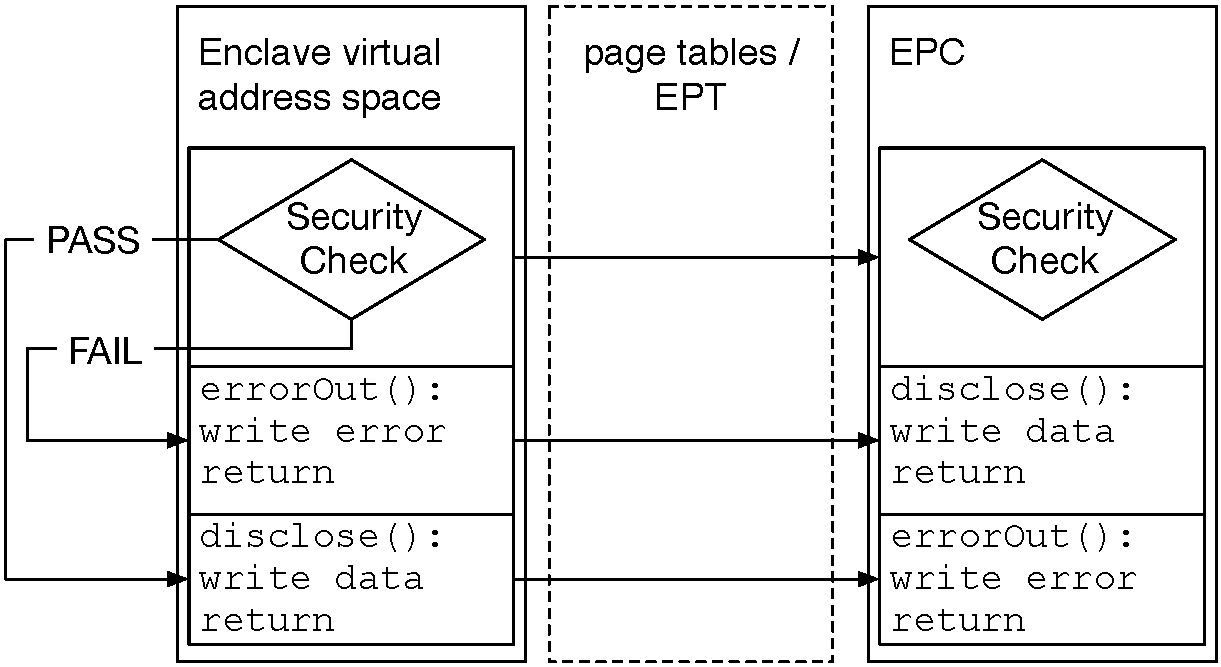
\includegraphics[width=85mm]{figures/sgx_mapping_attack.pdf}
  \caption{
    An example of a memory mapping attack, which is prevented by SGX. The
    enclave's author intends to disclose a piece of sensitive information only
    when a security check passes. Malicious system software maps the virtual
    address of the procedure called when the security check fails to an EPC
    page that contains the procedure that discloses the sensitive information,
    which is supposed to be called when the security check passes.
  }
  \label{fig:sgx_mapping_attack}
\end{figure}

For simplicity, we assume an enclave that performs a security check to decide
whether to disclose some sensitive information. Depending on the security
check's outcome, the enclave code either calls a \texttt{errorOut} procedure,
or a \texttt{disclose} procedure. We furthermore assume that each procedure's
code starts at a 4KB boundary, and takes up less than 4KB, so each procedure
fits in an EPC page. These requirements seem unrealistic, but the underlying
attack remains an issue in real applications.

In a memory mapping attack, malicious system software sets up the page tables
or EPT in such a way that the virtual address intended to store the
\texttt{errorOut} procedure is actually mapped to an EPC page that contains the
\texttt{disclose} procedure. Without any security measures in place, the
enclave would execute the \texttt{disclose} code and reveal sensitive
information, even though the security check fails.

The SGX security mechanisms, explained throughout the rest of this paper,
prevent enclave code execution if a memory mapping attack occurs. Therefore,
SGX prevents malicious system software from directly obtaining sensitive
information via memory mapping attacks.
